\documentclass[a4paper,11pt]{article}
\usepackage[utf8]{inputenc}
\usepackage{algorithmic}
\usepackage{algorithm}
\usepackage{pst-plot}
\usepackage{graphicx}
\usepackage{endnotes}
\usepackage{graphics}
\usepackage{floatflt}
\usepackage{wrapfig}
\usepackage{amsfonts}
\usepackage{amsmath}
\usepackage{verbatim}
\usepackage{hyperref}
\usepackage{multirow}
\usepackage{pdflscape}
\usepackage{wrapfig}
\usepackage{gensymb}

\usepackage{hyperref}
\hypersetup{pdfborder={0 0 0 0}}

\pdfpagewidth 210mm
\pdfpageheight 297mm 
\setlength\topmargin{0mm}
\setlength\headheight{0mm}
\setlength\headsep{0mm}
\setlength\textheight{250mm}	
\setlength\textwidth{159.2mm}
\setlength\oddsidemargin{0mm}
\setlength\evensidemargin{0mm}
\setlength\parindent{7mm}
\setlength\parskip{0mm}

\newenvironment{exercise}[3]{\paragraph{Exercise #1: #2 (#3pt)}\ \\}{
\medskip}
\newcommand{\question}[2]{\setlength\parindent{0mm}\ \\$\mathbf{Q_#1:}$ #2\ \\}

\author{\large{Ilya Kuzovkin, Raul Vicente}}
\title{\huge{Introduction to Computational Neuroscience}\\\LARGE{Practice III: Data Analysis - Spiking Data}}

\begin{document}
\maketitle

The last time we had a look at the continuous brain data: strength of the EEG signal was changing over the time. Another very popular form of data, mostly associated with the single neuron recordings, is \emph{spiking} data. The concept is very simple: we attach a sensor to the neuron and when the neuron fires we write "1" into our data file, otherwise we write "0". The resulting data shows us for each time point whether the neuron has fired or not.\\
\ \\
\textbf{Request}: Please record the time you will spend of this homework and add it to the report. This is just for me to balance the amount and the difficulty level of the exercises.\\
\ \\
\textbf{Dataset}

\begin{wrapfigure}{r}{0.3\textwidth}
	\centering
	\vspace{-12pt}
	
\includegraphics[width=0.15\textwidth]{orientationstimulus.jpg}
	\caption{Example of the stimulus. During the actual experiment the bars are moving.}
	\label{fig:stimulusexample}
	\vspace{-5pt}
\end{wrapfigure}
The dataset we will be working with has the spiking data recorded while the mouse was presented with a stimulus: moving bar on the screen, which can have different orientations. On Figure \ref{fig:stimulusexample} you can see an example: white and black bars are tilted (\emph{orientation}) and they are moving. The spiking activity is recorded from the 72 neurons and we want to find is whether different neurons react differently on the stimuli with different orientation. Have a look at Figure \ref{fig:orientationresponse} -- spiking pattern of this particular neuron seems to indicate that this neuron is more active when the bar is tilted $45\degree$ clockwise from the horizontal position. And its activity fades when the bar changes the orientation. We would like to rediscover from the data, than indeed different neurons respond differently to different orientations.
\begin{figure}[H]
	\centering
	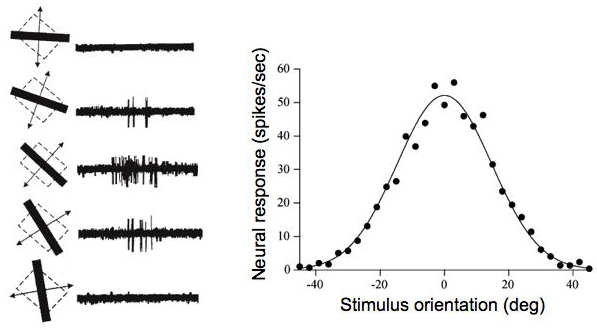
\includegraphics[width=0.8\textwidth]{orientation.jpg} 
	\caption{Neuronal response to different orientations of the bar.}
	\label{fig:orientationresponse}
\end{figure}
\textbf{NB:} Note that in the dataset we have 13 stimuli (13 orientations), but the first one should be ignored (it has orientation $-1\degree$). So you should use only the other 12.


\begin{exercise}{1}{Raster plot}{0.5}
Let us start by plotting some spiking data. Under the \texttt{data/lgn} folder you have recordings from 72 neurons of a mouse. \texttt{Matlab/Octave} users can use files in the \texttt{matlab} folder, the same data is available in the plain text format in the \texttt{plain} folder.

\texttt{Matlab} files have names \texttt{mlgnori\_NN.mat} where \texttt{NN} is the number of the neuron. When you load it to your environment you will find that each file has a structure with two elements: \texttt{spktimes} and \texttt{stim}. The first one is $M\times N \times T$ matrix where $M$ is the stimulus number, $N$ is the trial number at $T$ is the time in milliseconds. So this is a 3-dimensional matrix with values 0 (no spike) and 1 (spike). The second file describes the stimulus. Open it and you will see what information is in there.

If you do not use \texttt{Matlab}, then it is easier for you to use the plain text files. They have names \texttt{neuron\_NN} \texttt{\_stimulus\_SS.csv} where \texttt{NN} is the number of the neuron and \texttt{SS} is the number of the stimulus. Inside each file one line represents one trial. For each millisecond it has value 0 (no spike) or 1 (spike). Files with names \texttt{stimulus\_SS.csv} describe the stimulus: they hold four values:
\begin{enumerate}
\itemsep 0em
	\item Time before the stimulus (in seconds).
	\item Duration of the stimulus (in seconds).
	\item Time after the stimulus (in seconds).
	\item Orientation of the stimulus (in degrees).
\end{enumerate}
Your task is to take any of the neurons and plot all trials as a raster plot (see Figure \ref{fig:raster_plot}). You will notice that neuronal response to the stimulus varies a lot, this is why you usually need several trials.
\begin{figure}[H]
   \centering
   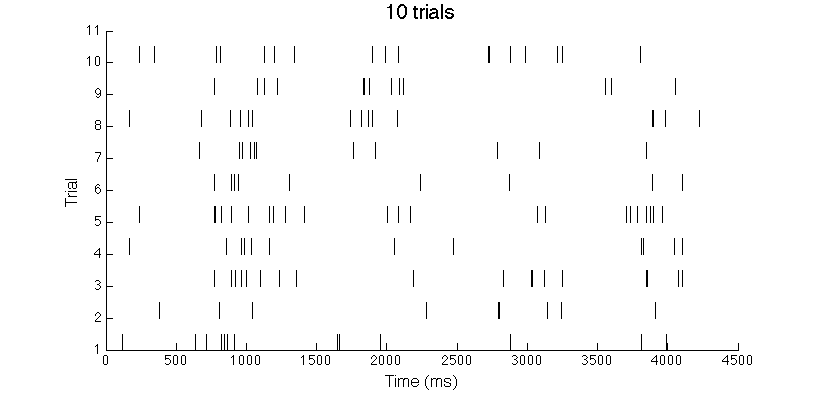
\includegraphics[width=0.7\textwidth]{raster10tr.png} 
   \caption{Raster plot of 10 trials on the same neuron.}
   \label{fig:raster_plot}
\end{figure}
On the $X$ axis we have time and on the $Y$ axis trials. A vertical bar indicates a spike. To draw a vertical line in \texttt{Matlab} you can use
\begin{verbatim}
	line([t t], [tr tr+0.5], 'Color', 'k');
\end{verbatim}
where \texttt{t} is the time and \texttt{tr} is the number of the trial.
\end{exercise}


\begin{exercise}{2}{More raster plots}{0.5}
The next step is to create two more raster plots. The first one will illustrate the behaviour of all the neurons under the same stimulus, while the other one will have responses of the same neuron but to the different stimuli.

First we need to average spiking data so that each neuron would be represented by one vector. Simplest way to do that is just to add trials together. Let us say that you have 10 trials, and each of them is a vector of 4500 time points. You just sum those vectors together to obtain one vector of length 4500. After that replace all values which are grater than 1 with 1.

Create the following two plots:
\begin{enumerate}
	\item Raster plot, where on $X$ axis we have time and on $Y$ axis we have all 72 neurons. Verticals bars are the responses to the same stimulus (choose any). Please note that in our dataset different recordings have different length, but this should not be a problem.
	\item Raster plot, where on $Y$ axis we have all 13 stimuli and bars are the responses from the same neuron (choose any) to those stimuli.
\end{enumerate}
\end{exercise}


\begin{exercise}{3}{Post-Stimulus Time Histogram (PSTH)}{0.5}
Another useful analysis tool is a histogram, where on $X$ axis we have time points (or time ranges) and on $Y$ axis the number of spikes that occurred during given time range. It is called \emph{Post-Stimulus Time Histogram (PSTH)}.
\begin{enumerate}
	\item Choose any neuron, any stimulus.
	\item Take an average over all trials as we did before.
	\item Choose time window, for example 20ms or 50ms.
	\item Plot a histogram, where on the $X$ axis we have time windows and on the $Y$ axis the number of spikes that occurred during that window.
\end{enumerate}
\end{exercise}


\begin{exercise}{4}{Tuning Curve}{0.5}
Yet another way of visualization is the \emph{tuning curve}. It is similar to the previous one, but now instead of the time we will plot a stimulus on the $X$ axis and number of spikes on the $Y$ axis.
\begin{enumerate}
	\item Choose any 3 neurons.
	\item For each neuron:
	\begin{enumerate}
		\item For each stimulus:
		\begin{enumerate}
			\item Calculate number of spikes during each trial into separate array. For example if we have 20 trials then this array will consist of 20 numbers.
			\item Calculate the average number of spikes per trial (use \texttt{mean} function).
			\item Calculate the standard deviation of the number of spikes (use \texttt{std} function).
		\end{enumerate}	
		\item You will have two arrays, both of length 12 (because we have 12 stimuli):
		\begin{enumerate}
			\item Average number of spikes for each stimulus.
			\item Standard deviation of number of spikes for each stimulus.
		\end{enumerate}
		\item Use function \texttt{errorbar(average\_numbers, standard\_deviations)} to plot the curve and standard deviation bars.
	\end{enumerate}
	\item The result should look something like the one you see on Figure \ref{fig:tuningcurve}.
\end{enumerate}

\begin{figure}[H]
   \centering
   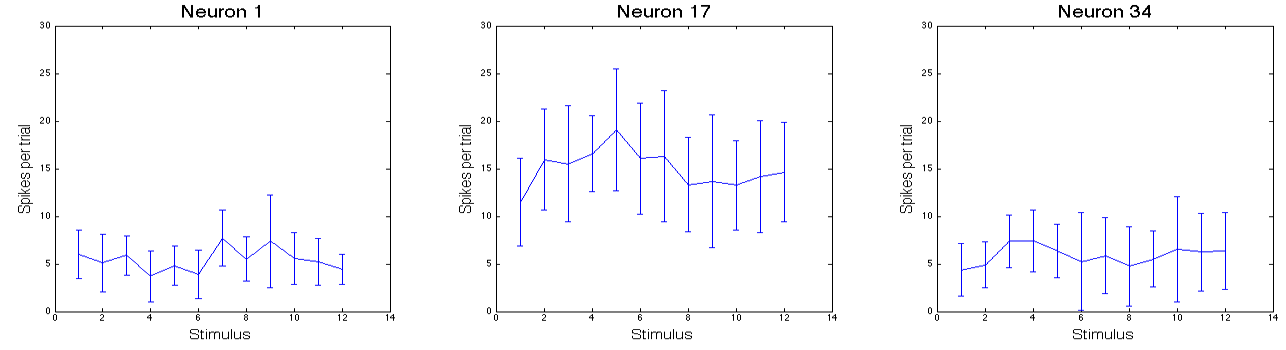
\includegraphics[width=0.8\textwidth]{tuningcurve.png} 
   \caption{Tuning curve with standard deviation bars.}
   \label{fig:tuningcurve}
\end{figure}

\end{exercise}

\begin{exercise}{5*}{Rose diagram}{0.5}
There is a really neat way to visualize the tuning curve. In fits especially well with the experiment we have at our hands. It is called \emph{rose chart} or \emph{angle histogram}. You can see an example on Figure \ref{fig:rosediag}. The idea is that the values are placed on the circumference on the circle and the length of the sector is determined by the number of times the value appears in the list. It is like a histogram drawn in circle.

In the most cases this is just a fancy way to draw a histogram, but in our case it allows to represent our data in much better way by placing orientations (stimuli) on the circe. For example on Figure \ref{fig:rosediag} we can clearly see that neuron 8 is reacts more to the orientation of $0\degree$, the neuron 6 is most active in the range of $270\degree$ to $330\degree$ and so on.

\begin{figure}[H]
   \centering
   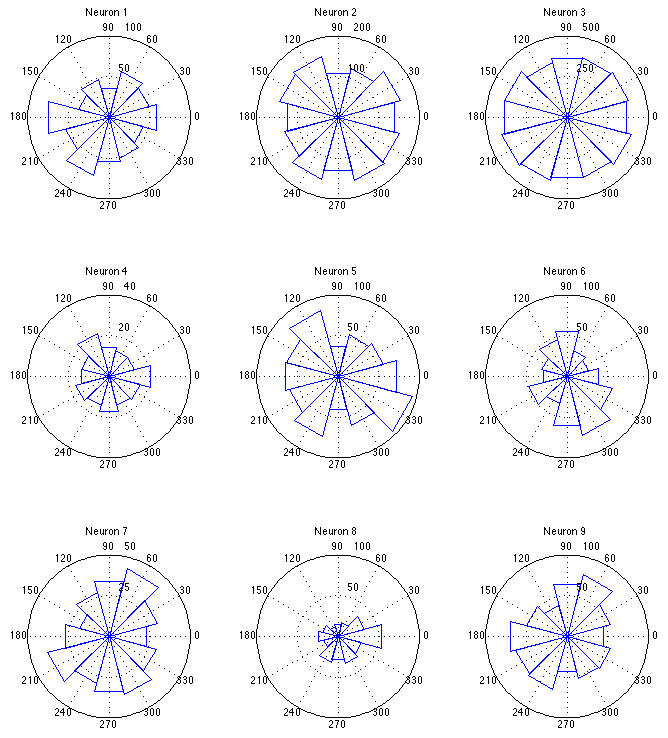
\includegraphics[width=0.7\textwidth]{rosediag.png} 
   \caption{Rose diagram: the number of spikes for each of 12 orientations.}
   \label{fig:rosediag}
\end{figure}

Your task is to produce similar plot for any 9 neurons. To produce a plot for one neuron do the following:
\begin{enumerate}
	\item Create an array \texttt{A} where for each spike you will store the orientation when the spike occurred.
	\item For each orientation (stimulus) do:
	\begin{enumerate}
		\item Count the number of times the neuron fired.
		\item Add to \texttt{A} current orientation as many times as the neuron fired.
	\end{enumerate}
	\item Draw the plot. In \texttt{Matlab} you can do:
	\begin{enumerate}
		\item Array with the angles of bins (needed for the \texttt{rose} function):\\ \texttt{angles = degtorad([0, 30, 60, 90, 120, 150, 180, 210, 240, 270, 300, 330]);}
		\item Call \texttt{rose(deg2rad(A), angles)}
	\end{enumerate}
\end{enumerate}
\end{exercise}


\begin{exercise}{6}{Receptive field}{1}
In general the \emph{receptive field} of a neuron is a region of space in which the presence of a stimulus will alter the firing of that neuron. By now you have a set of tools to analyse our spiking data and estimate the receptive fields of the neurons in the dataset we have. In our case the receptive field is the orientation of the bar on the screen (each of the neurons has a set of orientations it reacts to). Your task is to find 5 neurons with the most specific receptive fields. You can use any of the tools we have seen during this session or any other methods you find useful.

In your report please describe what you did, your findings and the list of 5 neurons with the most specific orientations.
\end{exercise}


\begin{exercise}{7*}{What else our neurons are tuned to?}{0.5}
In this session we have seen an example of how neurons are ``tuned" to respond to very specific stimuli. You task is to find  other interesting examples of stimuli our neurons are tuned to react to. Are there special neurons, which fire when you look at a human face? Neurons which react on the temperature? Hunger? Numbers?...
\end{exercise}



\ \\
\ \\
\ \\
\ \\
\ \\
Please submit a \texttt{pdf} report with answers to the questions and comments about your solutions. Also submit a code for the programming exercise(s). Pack those into \texttt{zip} archive and upload to the course web page.

\end{document}










